\documentclass[11pt,twoside,a4paper]{article}
% http://www-h.eng.cam.ac.uk/help/tpl/textprocessing/latex_maths+pix/node6.html symboles de math
% http://fr.wikibooks.org/wiki/Programmation_LaTeX Programmation latex (wikibook)
%=========================== En-Tete =================================
%--- Insertion de paquetages (optionnel) ---
\usepackage[english]{babel}
\usepackage{a4}	             % pour la taille   
\usepackage[T1]{fontenc}     % pour les font postscript
\usepackage{epsfig}          % pour gerer les images
%\usepackage{psfig}
\usepackage{amsmath, amsthm} % tres bon mode mathematique
\usepackage{amsfonts,amssymb}% permet la definition des ensembles
\usepackage{float}           % pour le placement des figure
\usepackage{verbatim}

\usepackage{longtable} % pour les tableaux de plusieurs pages

\usepackage[table]{xcolor} % couleur de fond des cellules de tableaux

\usepackage{lastpage}

\usepackage{multirow}

\usepackage{multicol} % pour {\'e}crire dans certaines zones en colonnes : \begin{multicols}{nb colonnes}...\end{multicols} 

% \usepackage[top=1.5cm, bottom=1.5cm, left=1.5cm, right=1.5cm]{geometry}
% gauche, haut, droite, bas, entete, ente2txt, pied, txt2pied
\usepackage{vmargin}
\setmarginsrb{1.0cm}{1.0cm}{1.0cm}{1.0cm}{15pt}{3pt}{60pt}{25pt}

\usepackage{lscape} % changement orientation page
%\usepackage{frbib} % enlever pour obtenir references en anglais
% --- style de page (pour les en-tete) ---
\pagestyle{headings}

% % % en-tete et pieds de page configurables : fancyhdr.sty

% http://www.trustonme.net/didactels/250.html

% http://ww3.ac-poitiers.fr/math/tex/pratique/entete/entete.htm
% http://www.ctan.org/tex-archive/macros/latex/contrib/fancyhdr/fancyhdr.pdf
\usepackage{fancyhdr}
\pagestyle{fancy}
% \newcommand{\chaptermark}[1]{\markboth{#1}{}}
% \newcommand{\sectionmark}[1]{\markright{\thesection\ #1}}
\fancyhf{}
\fancyhead[LE,RO]{\bfseries\thepage}
\fancyhead[LO]{\bfseries\rightmark}
\fancyhead[RE]{\bfseries\leftmark}
\fancyfoot[LE]{\thepage /\pageref{LastPage} \hfill
	DNA seen through the eyes of a coder
\hfill 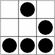
\includegraphics[width=0.5cm]{img/logo_glider.png} }
\fancyfoot[RO]{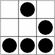
\includegraphics[width=0.5cm]{img/logo_glider.png} \hfill
	DNA seen through the eyes of a coder
\hfill \thepage /\pageref{LastPage}}
\renewcommand{\headrulewidth}{0.25pt}
\renewcommand{\footrulewidth}{0.50pt}
\addtolength{\headheight}{0.5pt}
\fancypagestyle{plain}{
	\fancyhead{}
	\renewcommand{\headrulewidth}{0pt}
}

%--- Definitions de nouvelles commandes ---
\newcommand{\N}{\mathbb{N}} % les entiers naturels


%============================= Corps =================================
\begin{document}

\setlength\parindent{0pt}

%% ~\\
\vfill

\begin{center}
	\textbf{\Large DNA seen through the eyes of a coder}~\\
	\textbf{or}~\\
	\textbf{\large If you are a hammer, everything looks like a nail}~\\
	~\\
	\texttt{http://ds9a.nl/amazing-dna/}
\end{center}

``\emph{This is one of the coolest things I've read in a while.} '' -- -- \texttt{jwz}~\footnote{\texttt{http://www.livejournal.com/users/jwz/}} ~\\

This is just some rambling by a computer programmer about DNA. I'm not a molecular geneticist. If you spot the inevitable mistakes, please mail me (\texttt{bert hubert}~\footnote{\texttt{http://ds9a.nl/}}) at \texttt{ahu@ds9a.nl}. ~\\

I'm not trying to force my view unto the DNA -- each observation here is quite 'uncramped'. To see where I got all this from, head to the bibliography. %% ~\\ 

\tableofcontents

\vfill

~\\

\clearpage

\section*{Updates\markboth{Updates}{Updates}}
\addcontentsline{toc}{section}{Updates}

3rd of January 2008: ~\\
A lot of updates are arriving since this page was linked on \texttt{Reddit.com}~\footnote{\texttt{http://reddit.com/}}, I'm currently evaluating and merging the suggested changes. Please do keep sending updates! ~\\

23rd of September 2006: ~\\
Small update on the number of genes. Some other updates have been sent to me over the past four years, and I'll try to work them in to the page. ~\\

16th of June 2002: ~\\
Added tiny piece on the \texttt{halting problem} and cancer. I think this is a new insight, but I'm not sure. On the todolist: Code reuse through alternative splicing. ~\\

18th of May 2002: ~\\
In the meantime some people who *are* geneticists have read this and have spotted and fixed some, but not many, mistakes. I recently added information on the cell as a state machine and on forking and forkbombs. ~\\

24th of May 2002: ~\\
Some clarifications from the great people on \#bioinformatics on OPN. Added a bunch of pictures to lighten up the page. Added piece on the \texttt{Central Dogma}. %% ~\\

\section*{The source code\markboth{The source code}{The source code}}
\addcontentsline{toc}{section}{The source code}

Is \texttt{here}~\footnote{\texttt{ftp://ftp.ensembl.org/pub/current\_genbank/homo\_sapiens/}}. This not a joke. We can wonder about the license though. Maybe we should ask the walking product of this source: \texttt{Craig Venter}~\footnote{\texttt{http://www.guardian.co.uk/Archive/Article/0,4273,4403109,00.html}}. The source can be viewed~\footnote{\texttt{http://www.ensembl.org/Homo\_sapiens/}} via a wonderful set of perl scripts called 'Ensembl'~\footnote{\texttt{http://www.ensembl.org/Homo\_sapiens/Download/}}. The human genome is about 3 gigabases long, which boils down to 750 megabytes. Depressingly enough, this is only 2.8 Mozilla browsers~\footnote{\texttt{http://ftp.mozilla.org/pub/mozilla/releases/}}. ~\\

DNA is not like C source but more like byte-compiled code for a virtual machine called 'the nucleus'. It is very doubtful that there is a source to this byte compilation -- what you see is all you get. ~\\

The language of DNA is digital, but not binary. Where binary encoding has 0 and 1 to work with (2 -- hence the 'bi'nary), DNA has 4 positions, T, C, G and A. ~\\

\begin{minipage}[ht]{10.75cm}	
	Whereas a digital byte is mostly 8 binary digits, a DNA 'byte' (called a 'codon') has three digits. Because each digit can have 4 values instead of 2, an DNA codon has 64 possible values, compared to a binary byte which has 256. ~\\
		
	A typical example of a DNA codon is 'GCC', which encodes the amino acid Alanine. A larger number of these amino acids combined are called a 'polypeptide' or 'protein', and these are chemically active in making a living being. ~\\
\end{minipage} \hfill \begin{minipage}[ht]{8.25cm}
	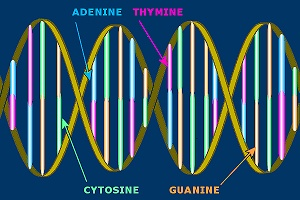
\includegraphics[width=8.0cm]{img/dna.jpg}
\end{minipage}

	See also \texttt{http://www.ultranet.com/\textasciitilde jkimball/BiologyPages/C/Codons.html}. %% ~\\ 

\section*{Position Independent Code\markboth{Position Independent Code}{Position Independent Code}}
\addcontentsline{toc}{section}{Position Independent Code}

Dynamically linked libraries (.so under Unix, .dll on Microsoft) code cannot use static addresses internally because the code may appear in different places in memory in different situations. DNA has this too, where it is called 'transposing code': ~\\

	\emph{Nearly half of the human genome is composed of transposable elements or jumping DNA. First recognized in the 1940s by Dr. Barbara McClintock in studies of peculiar inheritance patterns found in the colors of Indian corn, jumping DNA refers to the idea that some stretches of DNA are unstable and "transposable," ie., they can move around -- on and between chromosomes. }~\\ 	
	\texttt{http://www.ornl.gov/hgmis/resource/people.html} %% ~\\
	
\section*{Conditional compilation\markboth{Conditional compilation}{Conditional compilation}}
\addcontentsline{toc}{section}{Conditional compilation}

\begin{minipage}[ht]{7.25cm}
	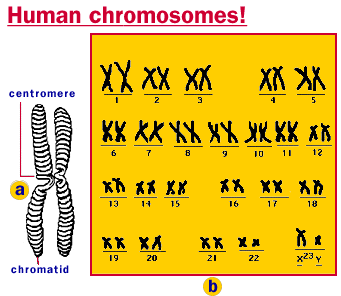
\includegraphics[width=7.0cm]{img/human_chrom.png}
\end{minipage} \hfill \begin{minipage}[ht]{11.75cm}
	Of the \texttt{20,000 to 30,000 genes}~\footnotemark now thought to be in the human genome, most cells express only a very small part -- which makes sense, a liver cell has little need for the DNA code that makes neurons. ~\\

	But as almost all cells carry around a full copy ('distribution') of the genome, a system is needed to \#ifdef out stuff not needed. And that is just how it works. The genetic code is full of \#if/\#endif statements. ~\\
\end{minipage}
\footnotetext{\texttt{http://www.commondreams.org/views01/0212-02.htm}}

This is why 'stem cells'~\footnote{\texttt{http://www.ultranet.com/\textasciitilde jkimball/BiologyPages/S/Stem\_Cells.html}}  are so hot right now -- these cells have the ability to differentiate into everything. The code hasn't been \#ifdeffed out yet, so to speak. ~\\

Stated more exactly, stem cells do not have everything turned on -- they are not at once liver cells and neurons. Cells can be likened to state machines, starting out as a stem cell. Over the lifetime of the cell, during which time it may clone ('fork()') many times, it specializes. Each specialization can be regarded as chosing a branch in a tree. ~\\

Each cell can make (or be induced to make) decisions about its future, which each make it more specialized. These decisions are persistent over cloning using transcription factors and by modifying the way DNA is stored spacially ('steric effects'). ~\\

A liver cell, although it carries the genes to do so, will generally not be able to function as a skin cell. There are some indications out there that it is possible to 'breed' cells 'upwards' into the hierarchy, making them pluripotent. See also this article~\footnote{\texttt{http://www.sciencedaily.com/releases/2002/01/020131074645.htm}}. %% ~\\

\clearpage

\section*{Dead code, bloat, comments ('junk dna')\markboth{Dead code, bloat, comments ('junk dna')}{Dead code, bloat, comments ('junk dna')}}
\addcontentsline{toc}{section}{Dead code, bloat, comments ('junk dna')}

\begin{minipage}[ht]{9.25cm}
	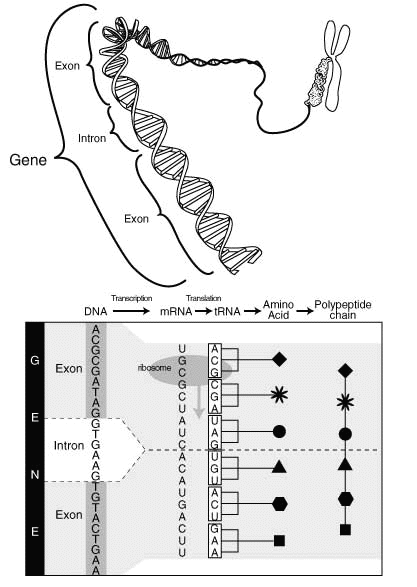
\includegraphics[width=9.0cm]{img/intron.png}
\end{minipage} \hfill \begin{minipage}[ht]{9.75cm}
	The genome is littered with old copies of genes and experiments that went wrong somewhere in the recent past -- say, the last half a million years. This code is there but inactive. These are called the 'pseudo genes'. ~\\

	Furthermore, 97\% of your DNA is commented out. DNA is linear and read from start to end. The parts that should not be decoded are marked very clearly, much like C comments. The 3\% that is used directly form the so called 'exons'. The comments, that come 'inbetween' are called 'introns'. ~\\
	
	These comments are fascinating in their own right. Like C comments they have a start marker, like /*, and a stop marker, like */. But they have some more structure. Remember that DNA is like a tape -- the comments need to be snipped out physically! The start of a comment is almost always indicated by the letters 'GT', which thus corresponds to /*, the end is signalled by 'AG', which is then like */. ~\\
	
	However because of the snipping, some glue is needed to connect the code before the comment to the code after, which makes the comments more like html comments, which are longer: '<!--' signifies the start, '-->' the end. ~\\
	
	So an actual stretch of DNA with exons and introns might look like this:
\end{minipage}

\begin{center}
	\begin{verbatim}
		ACTUAL CODE<!-- blah blah blah blah ---- blah -->ACTUAL CODE
		  |         |            |           |        |        |
		exon 1    acceptor    intron 1     branch   donor   exon 2
		     (start of comment)                 (end of comment)
	\end{verbatim}
\end{center}

The start of the comment is clear, which is then followed by a lot of non-coding DNA. Somewhere very near the end of the comment there is a 'branch site', which indicates that the comment will end soon. Then some more comment follows, and then the actual terminator. ~\\

The actual cutting of the comments happens after the DNA has been transcribed into RNA and is performed by looping the comment and bringing the pieces of actual code close together. Then the RNA is cut at the 'branch site' near the end of the comment, after which the 'acceptor' (comment start) and 'donator' (comment end) are connected to eachother. ~\\

Now, what are these comments good for? That discussion is part of a \texttt{holy war}~\footnote{\texttt{http://www.tuxedo.org/\textasciitilde esr/jargon/html/entry/holy-wars.html}} that can rival the vi/emacs one. When comparing different species, we know that some introns show fewer code changes than the neighboring exons. This suggests that the comments are doing something important. ~\\

There are lots of possible explanations for the massive amount of non-coding DNA -- one of the most appealing (to a coder) has to do with 'folding propensity'. DNA needs to be stored in a highly coiled form, but not all DNA codes lend themselves well to this. --- This may remind you of \texttt{RLL or MFM coding}~\footnote{\texttt{http://www-2.cs.cmu.edu/\textasciitilde 412/applications/ln/lecture16.html}}. On a hard disk, a bit is encoded by a polarity transition or the lack thereof. A naive encoding would encode a 0 as 'no transition' and 1 as 'a transition'. ~\\

Encoding 000000 is easy -- just keep the magnetic phase unchanged for a few micrometers. However, when decoding, uncertainty creaps in -- how many micrometers did we read? Does this correspond to 6 zeroes or 5? To prevent this problem, data is treated such that these long stretches of no transitions do not occur. ~\\

If we see 'no transition,no transition,transition,transition' on disk, we can be sure that this corresponds to '0011' -- it is exceedingly unlikely that our reading process is so imprecise that this might correspond to '00011' or '00111'. So we need to insert spacers so as to prevent too little transitions. This is called 'Run Lengh Limiting' on magnetic media. --- \textbf{The thing to note} is that sometimes, transitions need to be inserted to make sure that the data can be stored reliably. Introns may do much the same thing by making sure that the resulting code can be coiled properly. ~\\

However, this area of molecular biology is a minefield! Huge diatribes rage about variants with exciting names like 'introns early' or 'introns late', and massive words like 'folding propensity' and 'stem-loop potential'. I think it best to let this discussion rage on a bit. ~\\

\emph{A fascinating link of uncertain scientific value is \texttt{http://post.queensu.ca/\textasciitilde forsdyke/introns.htm}. } %% ~\\

\section*{fork() and fork bombs ('tumors')\markboth{fork() and fork bombs ('tumors')}{fork() and fork bombs ('tumors')}}
\addcontentsline{toc}{section}{fork() and fork bombs ('tumors')}

\begin{minipage}[ht]{13.75cm}
	Like with unix, cells are not 'spawned' -- they are forked. All cells started out from your ovum which has forked itself many times since. Like processes, both halves of the fork() are (mostly) identical to begin with, but they may from then on decide to do different things. ~\\

	As with unix, great problems arise when cells keep on forking. They quickly exhaust resources, sometimes leading to death. This is called a tumor. The cell is riddled with 'ulimits' and 'watchdogs' to prevent this sort of thing from happening. The number of divisions is limited by \texttt{Telomere shortening}~\footnotemark, for example. ~\\

	A cell cannot clone unless very stringent conditions are met -- a 'secure by default'~\footnotemark configuration. It is only when these safeguards fail that tumors can grow. Like with computer security, it is hard to strike a balance between security ('no cells can divide') and usability. ~\\

	Compare this to the well known \texttt{Halting Problem}~\footnotemark, first described by the founder of Computer Science, \texttt{Alan Turing}~\footnotemark. Perhaps it is as impossible to predict if a program will ever finish as it is to create a functional genome that cannot get cancer? %% ~\\
\end{minipage} \hfill \begin{minipage}[ht]{5.25cm}
	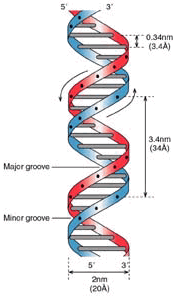
\includegraphics[width=5.0cm]{img/helix.png}
\end{minipage}
\footnotetext{\texttt{http://www.ellison-med-fn.org/emf\_award.jsp?award\_id=10}}
\footnotetext{\texttt{http://www.openbsd.org/}}
\footnotetext{\texttt{http://www.cs.washington.edu/homes/csk/halt.html}}
\footnotetext{\texttt{http://www.turing.org.uk/turing/}}

\section*{Mirroring, failover\markboth{Mirroring, failover}{Mirroring, failover}}
\addcontentsline{toc}{section}{Mirroring, failover}

Each DNA Helix is redundant in itself -- you can see the genome as a twisted ladder whereby each spoke contains two bases -- hence the word 'basepair'. If one of these bases is missing, it can be derived from the one on the other side. T always binds to A, C always to G. So, we can state that the genome is mirrored within the helix. 'RAID-1' so to speak. ~\\

Furthermore, there are two copies of each chromosome present -- one from each parent, with the notable exception of the Y chromosome, which is only present in males. The actual details are complicated -- but most genes are thus present twice. In case one is broken or unusefully mutated, the other independent copy is still there. This is what we would normally call 'failover'. ~\\

\section*{Cluttered APIs, dependency hell\markboth{Cluttered APIs, dependency hell}{Cluttered APIs, dependency hell}}
\addcontentsline{toc}{section}{Cluttered APIs, dependency hell}

As proteins interact in the cell, they rely on eachothers' characteristics. It has just been shown that proteins that interact with a lot of other proteins cannot evolve, or at least, only do so at a very slow rate. See Nature, 28 June 2001, and M. Kimura, T. Ohta, Science, 26 April 2002. ~\\

They propose that this is because of great internal dependencies which inhibit the changing of the 'contract' of the protein. It is also noted that evolution does take place, but very slowly as both parts of the dependency need to evolve in a compatible way at the same time. %% ~\\

\section*{Viruses, worms\markboth{Viruses, worms}{Viruses, worms}}
\addcontentsline{toc}{section}{Viruses, worms}

Somebody recently proposed in a discussion that it would be really cool to hack the genome and compromise it so as to insert code that would copy itself to other genomes, using the host-body as its vehicle. 'Just like the nimda worm!' ~\\ 	

He shortly thereafter realised that this is exactly what biological viruses have been doing for millions of years. And they are exceedingly good at it. ~\\

A lot of these viruses have become a fixed part of our genome and hitch a ride with all of us. To do so, they have to hide from the virus scanner which tries to detect foreign code and prevent it from getting into the DNA. %% ~\\

\section*{The Central Dogma: .c -> .o -> a.out/.exe\markboth{The Central Dogma}{The Central Dogma}}
\addcontentsline{toc}{section}{The Central Dogma}

When scientists were still discovering the basics of genetics they were faced with lots of different chemicals but the correlation was unclear. When it became clear what comes from what it was hailed as a great triumph and called 'The Central Dogma'. ~\\

This dogma tells us that DNA is used to make RNA and that RNA is used to make proteins, which is like saying that from a .c file comes a .o object file, which can be compiled into an executable (a.out/exe). It also tells us that this is the only order in which information flows. ~\\

Now, the Central Dogma has recenly been tarnished somewhat. Like any billion year old coding project, a lot of hacking has been going on, and sometimes information flows the other way. Sometimes RNA patches the DNA and at other times, the DNA is modified by proteines created earlier. ~\\

But generally, the dependencies are clear, so the Central Dogma remains important. %% ~\\

\section*{Binary patching aka 'Gene therapy'\markboth{Binary patching aka 'Gene therapy'}{Binary patching aka 'Gene therapy'}}
\addcontentsline{toc}{section}{Binary patching aka 'Gene therapy'}

\begin{minipage}[ht]{7.25cm}
	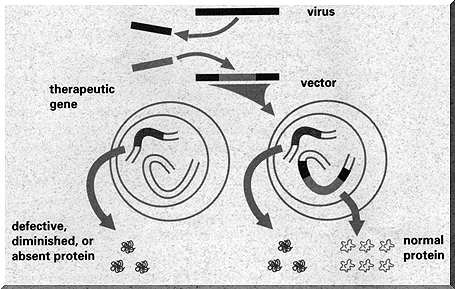
\includegraphics[width=7.0cm]{img/genetherapy1big.png}
\end{minipage} \hfill \begin{minipage}[ht]{11.75cm}
	We can fiddle easily enough with DNA. There are companies to which you can send an ASCII file with DNA characters, and they will synthesise the corresponding 'output' for you. We can also splice DNA into developing animals and plans. ~\\

	It is far harder to 'patch the running executable', as any programmer can attest. It is just like that with the genome. To change a running copy ('a human'), you need to edit each and every relevant copy of the gene you want to patch. ~\\
\end{minipage}

For many years, medical science has tried to patch people with SCID, or 'Severe Combined Immunodefeciency', which is a very nasty disease which in effect disables the immune system -- leading to very ill patients. It has been clear for quite a while now which letters in the DNA need to be fixed in order to cure these people. ~\\

Many attempts where made to patch running people, using viruses that insert new DNA into living organisms, but this proved to be very hard. The genome is guarded far too well for such a simple approach to work -- cells guard their code better than Microsoft! ~\\

However, recently the right virus was found which was able to breach the protection of the genome and fix the broken characters, leading to \texttt{apparently healthy people}~\footnote{\texttt{http://news.bbc.co.uk/hi/english/health/newsid\_1906000/1906999.stm}}. %% ~\\

\section*{Bug Regression\markboth{Bug Regression}{Bug Regression}}
\addcontentsline{toc}{section}{Bug Regression}

When fixing a bug in a computer program, we often introduce new bugs in the course of doing so. The genome is rife with this thing. A lot of African Americans are immune to Malaria but instead suffer from sickle cell anemia: ~\\

	\emph{In tropical regions of the world where the parasite-borne disease malaria is prevalent, people with a single copy of a particular genetic mutation have a survival advantage.} ~\\
	\emph{[...]} ~\\
	\emph{While inheriting one copy of the mutation confers a benefit, inheriting two copies is a tragedy. Children born with two copies of the genetic mutation have sickle cell anemia, a painful disease that affects the red blood cells.} ~\\
	\texttt{http://www.fda.gov/fdac/features/496\_sick.html} ~\\

There are quite a few examples of this happening. See also the wonderful book \texttt{'Genome' by Matt Ridley}~\footnote{\texttt{http://www.amazon.com/exec/obidos/ASIN/0060932902}}. %% ~\\

\section*{Reed-Solomon codes: 'Forward Error Correction'\markboth{Reed-Solomon codes: 'Forward Error Correction'}{Reed-Solomon codes: 'Forward Error Correction'}}
\addcontentsline{toc}{section}{Reed-Solomon codes: 'Forward Error Correction'}

\begin{minipage}[ht]{7.25cm}
	
\includegraphics[width=7.0cm]{img/nucleotides.jpg}
\end{minipage} \hfill \begin{minipage}[ht]{11.75cm}
	Like computer storage, DNA (and its intermediate 'RNA') can get corrupted. To protect against common 'single bit errors', the encoding from individual DNA letters to proteins is degenerate. There are 4 RNA characters, U, C, G and A -- in other words, a 'byte' is 2 bits long. Three characters correspond to an amino acid. ~\\
\end{minipage}

6 bits could conceivably map to 64 amino acids, yet there are only 20 in use. For example, UCU, UCC, UCA and UCG all encode for 'Serine', whereas only UGG maps to 'Tryptophan'. ~\\

Now, it turns out that some likely 'typos' (UCU -> UCC) in the encoding lead to an identical amino acid being expressed. For more about this fascinating phenomenon, read \texttt{'Metamagical Themas' by Douglas Hofstadter}~\footnote{\texttt{http://www.amazon.com/exec/obidos/ASIN/0465045669}}. %% ~\\

\section*{Holy Code: /* you are not expected to understand this */\markboth{Holy Code}{Holy Code}}
\addcontentsline{toc}{section}{Holy Code}

Some code is sacred. We may not remember who wrote it, or why -- we just know that it works. The guy who thought it up may have left the company already. Such code is not to be tinkered with. ~\\

DNA knows the concept of the 'molecular clock'. Some parts of the genome are actively changing and some parts are sacrosanct. A good example of the latter are the Histone genes H3 and H4. ~\\

These genes are fundamental to the actual storage of the genome and are thus of paramount importance. Any failure in this code rapidly leads to a non-functioning organism. ~\\

So it is to be expected that this code isn't tinkered with and that turns out the case. The H3 an H4 genes have a *zero* effective mutation rate in humans. But it goes far beyond that. You share almost the exact same code with anything from chickens to grass or moulds. ~\\

\begin{center}
	{\footnotesize RATES OF NUCLEOTIDE SUBSTITUTION PER SITE PER \textbf{1000 MILLION YEARS} BETWEEN VARIOUS HUMAN AND RODENT PROTEINS-CODING GENES WITH DIVERGENCE SET AT 80 MILLION YEARS BASED ON FOSSIL EVIDENCE:}
	\begin{tabular}[t]{ p{3cm} p{3cm} p{3cm} }
		gene				&	Number of codons	&	Effective rate	\\
		histone 3			&	135					&	0.00			\\
		histone 4			&	101					&	0.00			\\
		insulin				&	51					&	0.13			\\
		gamma interferon	&	136					&	2.79			\\
	\end{tabular}
	\texttt{http://www.staffs.ac.uk/schools/sciences/biology/Handbooks/evolseqphylo.htm}
\end{center}

Now, it does appear that there are two ways the genome can make sure that code does not mutate. The first way is described above: use amino acids that are highly degenerate and making sure that those typos that DO occur result in the same output. ~\\

Furthermore, genes can be copied earlier or later in the cell's reproductive process, leading to more or less favourable copying conditions. Many more of such conditions apply. --- It appears as if H3 and H4 were authored very carefully as they do have a lot of 'synonymous changes', which through the clever techniques described above do not lead to changes in the output. %% ~\\

\section*{Framing errors: start and stop bits\markboth{Framing errors}{Framing errors}}
\addcontentsline{toc}{section}{Framing errors}

\begin{verbatim}
			...0 0000 0001   0000 0010  0000 0011 0...
\end{verbatim}

This clearly describes the 8 bit values 1, 2 and 3. The spaces I added make it clear where a byte starts and stops. Many serial devices employ stop and start bits to encode where you start reading. If we shift this sequence slightly:
\begin{verbatim}
			...00 0000 0010   000 00100  000 00110 ...
\end{verbatim}

It suddenly reads 2, 4, 6! To prevent this from happening in DNA there are elaborate signals that tell the cell where to start reading. Interestingly, there are pieces of genome that can be read from multiple starting points, and produce useful (but different) results either way. That is what I call a cool hack! ~\\

Each way a strand of DNA can be read is called an \texttt{Open Reading Frame}~\footnote{\texttt{http://bioweb.uwlax.edu/GenWeb/Molecular/Seq\_Anal/Translation/translation.html}} and there are generally 6, 3 each way. %% ~\\

\section*{Massive multiprocessing: each cell is a universe\markboth{Massive multiprocessing}{Massive multiprocessing}}
\addcontentsline{toc}{section}{Massive multiprocessing}

Now, DNA is not like a computer programming language. It really isn't. But there are some whopping analogies. We can view each cell as a CPU, running its own kernel. Each cell has a copy of the entire kernel, but choses to activate only the relevant parts. Which modules or drivers it loads, so to speak. ~\\

If a cell needs to do something ('call a function'), it whips up the right piece of the genome and transcribes it into RNA. The RNA is then translated into a sequence of amino acids, which together make up a protein the DNA coded for. Now for the really cool bit :-) ~\\

\begin{minipage}[ht]{12.75cm}
	This protein is tagged with a shipping address. This is a marker consisting of several amino acids which tell the rest of the cell where this protein needs to go. There is machinery which acts on these instructions, and delivers the protein, which is potentially on the outside of the cell. ~\\

	The delivery instruction is then stripped off and several post processing steps may be performed, possibly activating the protein -- which is good, because you may not want to transport an active protein through places where it should not do work. ~\\
\end{minipage} \hfill \begin{minipage}[ht]{5.10cm}
	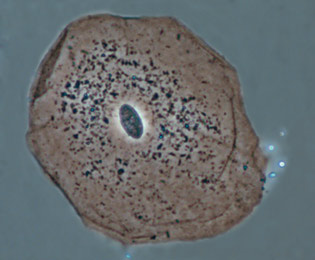
\includegraphics[width=5.0cm]{img/cell.jpg}~\\
	A Cell
\end{minipage}

\section*{Self hosting \& bootstrapping\markboth{Self hosting \& bootstrapping}{Self hosting \& bootstrapping}}
\addcontentsline{toc}{section}{Self hosting \& bootstrapping}

If we were to destroy all existing C compilers on the planet and leave only the code for one, we would be in great trouble. Yes, we have the C code to a C compiler, but we need a C compiler to compile it! ~\\

In actual fact, this was solved by not writing the first C compiler in C (duh), but in a language that was available already: B. See here~\footnote{\texttt{http://cm.bell-labs.com/cm/cs/who/dmr/chist.html}} for details about 'bootstrapping'. ~\\

The same holds for the genome. To create a new 'binary' of a specimen, a *living* copy is required. The genome needs an elaborate toolchain in order to deliver a living thing. The code itself is impotent. This toolchain is commonly called 'your parents'. ~\\

It appears that RNA, which is an intermediate code between DNA and a protein, may have been the 'B' for DNA. Which begs the question where RNA came from. It is very interesting to note that extra-terrestial objects often contain amino acids! See \texttt{http://www.google.com/search?hl=en\&q=amino+acids+meteorites} %% ~\\

\section*{The Makefile\markboth{The Makefile}{The Makefile}}
\addcontentsline{toc}{section}{The Makefile}

\begin{minipage}[ht]{8.10cm}
	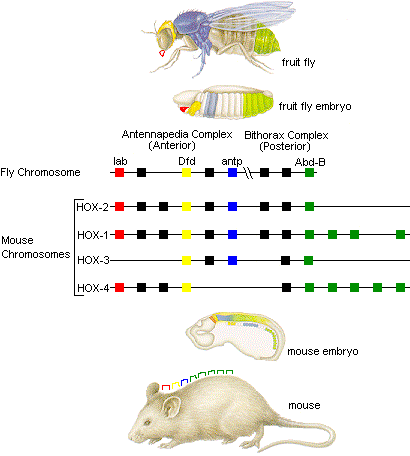
\includegraphics[width=8.0cm]{img/homeobox.png}
\end{minipage} \hfill \begin{minipage}[ht]{12.75cm}
	Organisms typically start out as a single cell, which as said before contains two entire copies of the genome. The big tarfile so to speak, with all files extracted, ready to go. Now what? ~\\

	Enter the \texttt{Homeobox genes}~\footnotemark. Cells must be copied and assigned a purpose. The Homebox genes start out by laying a 'top to bottom' dependency which reads 'start with the head'. In order to make this happen, a chemical gradient is created by which cells can sense where they are, and decide if they need to do things useful for building a head, or for building a primordial notochord. ~\\
	
	Only discovered in 1983, the Homebox genes are a very exciting area of research right now. It is interesting to note that like a Makefile, 'HOX' genes only trigger things in other genes and don't materially build things themselves. ~\\
\end{minipage}
\footnotetext{\texttt{http://www.people.virginia.edu/\textasciitilde rjh9u/homeo.html}}

The homebox 'syntax' appears to be very 'holy' in the sense described above. What happens if you copy paste the 'legs selector' part of a mouse HOX gene into the fruitfly Homebox: ~\\

	\emph{'In fact, when the mouse Hox-B6 gene is inserted in Drosophila, it can substitute for Antennapedia and produce legs in place of antennae'} ~\\
	\texttt{http://www.ultranet.com/\textasciitilde jkimball/BiologyPages/H/HomeoboxGenes.html} ~\\

The fruitfly and human genomes did not branch just millions of years ago but hundreds of millions of years ago. And you can copy paste parts ('Selectors' in the genetic language) of the Makefile and it still clicks. Please note that the 'build a leg' routine in a fruitfly is of course radically different from that in a mouse, but the 'selector' correctly triggers the right instructions. ~\\

\clearpage

\section*{Further reading\markboth{Further reading}{Further reading}}
\addcontentsline{toc}{section}{Further reading}

\emph{Genome}~\footnote{\texttt{http://www.amazon.com/exec/obidos/ASIN/0060932902}} by Matt Ridley ~\\
An amazing account of an effect each chromosome has on our lives. Very readable yet strict in not 'dumbing down' the theory. Contains an impressive set of references. ~\\

Source of many of the more impressive examples found on this page. ~\\

And to help Matt along in the quest he clearly sets out in his book, I would like to state quite clearly: ~\\

\begin{center} \textbf{Genes are not there to cause diseases} \end{center} ~\\

\emph{Human Molecular Genetics, second edition}~\footnote{\texttt{http://www.amazon.com/exec/obidos/ASIN/0471330612}} by Tom Strachan and Andrew P. Read ~\\
Neatly fills the gap between 'primary literature' (ie, peer reviewed academic magazines and papers) and introductory textbooks. I'm litteraly dragging myself through this book, constantly looking things up in order to understand everything. If you really want to know the details about introns, exons, RNA in all its variants, how genes cause and prevent diseases, this is the book. ~\\

\emph{The Selfish Gene}~\footnote{\texttt{http://www.amazon.com/exec/obidos/ASIN/0192860925}} by Richard Dawkins ~\\
Richard Dawkins~\footnote{\texttt{http://www.amazon.com/exec/obidos/search-handle-url/index=books\&field-author=Dawkins, Richard/}} is the Richard Stevens~\footnote{\texttt{http://www.amazon.com/exec/obidos/search-handle-url/index=books\&field-author=Stevens, Richard/}} of evolution theory. Both have contributed practical work but are most famous for their crystal clear expositions of existing theory, opening up the world they describe to an audience of millions. ~\\

In this book, Dawkins explains evolution from a 'gene' standpoint rather then from a 'species' standpoint. It turns out to make a lot more sense this way and helps understand how genes power you, and not the other way around. It is not that genes help you do what you want to do, you ARE the genes. ~\\

Also explains a lot about how genes work along the way. ~\\

\emph{The Blind Watchmaker : Why the Evidence of Evolution Reveals a Universe Without Design}~\footnote{\texttt{http://www.amazon.com/exec/obidos/ASIN/0393315703}} by Richard Dawkins ~\\
Again a book by Dawkins. More about evolution than about genes but clearly explains how evolution can be responsible for the intricate design found in many living things. ~\\

Again very readable and fascinating on every level. ~\\

\emph{Metamagical Themas}~\footnote{\texttt{http://www.amazon.com/exec/obidos/ASIN/0465045669}} by Douglas Hofstadter ~\\
This is an 'idea' book. It is filled to the brim with ideas, they simply ooze out of the pages. Many of these ideas are about information theory, genetics, life, intelligence, music, mathematics and people. ~\\

Clearly not a genetic textbook but has been influential in imbueing enthousiasm for all things genetic in many people. Can often be found dirt cheap in second hand bookstores. ~\\

Recommended. ~\\

\clearpage

%% \section*{Bibliography\markboth{Bibliography}{Bibliography}}
%% \addcontentsline{toc}{section}{Bibliography}
%% \bibliography{DNAthroughEyeOfaCoder}
%% \bibliographystyle{frplain} % plain or frplain

\end{document}
